\section{Association Rules Discovery}
\begin{itemize}
	\item Goal: discover \textbf{correlation among attributes} or other relationships in large databases.
	\item Use-case: Market Basket Analysis, cross/up-selling
	\item \textbf{Unsupervised learning}: no dependent variable defined, no labeled training data.
\end{itemize}

\subsection{Terminology}

\paragraph{Rule} if $A$ and $B$ then $C$ and $D$. denote as $R: A,B \Rightarrow C,D$. It only describes \textbf{correlation}, not causality. 



\paragraph{Transaction Database} an instance/observation is a transaction. Each \textbf{attribute} in the database is converted to \textbf{binary flags 0/1}. 
\paragraph{Item} single element/attribute. eg: Milk/Bread
\paragraph{Itemset} a set of items. eg: {Milk, Bread, Butter}
\paragraph{Frequent Itemset} the itemset $I$ that meets the \textbf{minimum support}. $$supp(I) \geq \min supp$$
\paragraph{Support}
\begin{itemize}
	\item support of \textbf{an item set}: \textbf{relative frequency} of the transactions that contain the item-set in \textbf{all transactions}
	\item support of \textbf{a rule}: the support of all item sets it contains. 
	$$supp(A,B \Rightarrow C,D) = supp(\{A,B,C,D\})$$
	The \textbf{order, the arrow} of the rule \textbf{doesn't matter in computing support}.
	$$supp(\text{Milk} \Rightarrow \text{Bread}) = supp(\{\text{Milk, Bread}\}) = supp(\{\text{Bread} \Rightarrow \text{Milk}\})$$
	
	\item support \textbf{estimation}: lower bound + upper bound. 
	\begin{itemize}
		\item lower bound: the support of a subset is always higher than its superset. \textbf{subset property}, every subset of a frequent set is frequent. 
		$$supp(\{B,C\}) \geq supp(\{A,B,C,D\})$$
		\item upper bound: use Venn-Diagramm.
	\end{itemize}
\end{itemize}

\paragraph{Confidence of a Rule} the likeliness to apply to the dataset. $\rightarrow$ the probability that X and Y coexist given that X exists.
$$conf(R: X \Rightarrow Y) = \frac{supp(X \cup Y)}{supp(X)}$$

$$conf(\{\text{Milk,Bread}\} \Rightarrow \{\text{Butter}\}) = \frac{supp(\{\text{Milk, Bread, Butter}\})}{supp(\{\text{Milk, Bread}\})}$$

\paragraph{Strong Rule} association rules with \textbf{minimum support \& confidence}.

\paragraph{Lift of a Rule} indicates \textbf{by how much (ratio)} the \textbf{confidence of a rule} surpasses the \textbf{expected value}. 
$$Lift(R: X \Rightarrow Y) = \frac{conf(R)}{expConf(R)} = \dfrac{\frac{supp(X \cup Y)}{supp(X)}}{supp(Y)} = \frac{supp(X \cup Y)}{supp(X)\cdot supp(Y)}$$

\subparagraph{Interpretation of Lifts}
\begin{itemize}
	\item lift < 1: X has \textbf{positive} effect on Y. Item-sets X and Y appears \textbf{more frequent than expected value}.
	\item lift = 1: X and Y are \textbf{independent}. X has \textbf{no effect} on Y.
	\item lift > 1: X has \textbf{negative} effect on Y. Item-sets X and Y appears \textbf{less frequent than expected value}.
\end{itemize}


\subsection{A priori Algorithm: Generation of Itemsets and Rules}

\begin{itemize}
	\item Idea: if X is a frequent k-item set, then all (k-1)-item subsets of X have to be frequent item sets as well.
	
	$\rightarrow$ iteratively compute frequent item sets, compute k-item sets by merging (k-1)-item sets.
	
	\item Process: 
	\begin{enumerate}[label= \protect \circled{\arabic*} ]
		\item Generation of \textbf{Item sets}: 
		\begin{itemize}
			\item start with item sets in \textbf{size 1}.
			\item only select those that \textbf{exceeds minimum support} $\rightarrow$ frequent.
			\item iteratively build item sets in larger sizes based on previous sizes. 
		\end{itemize}
	\begin{figure}[H]
		\centering
		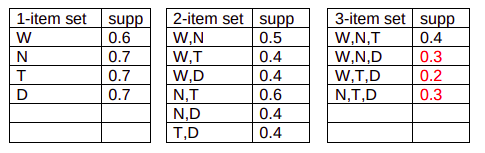
\includegraphics[width=0.5\textwidth]{itemset.png}
	\end{figure}
		\item Generation of \textbf{Rules} based on frequent item sets:
		\begin{itemize}
			\item start with rules with only \textbf{1 item on the right}. 
			\item rule $X \Rightarrow Y$ is different from $Y \Rightarrow X$. Compute \textbf{both directions}. 
			\item only select rules that \textbf{exceeds minimum confidence}. 
			\item evaluate rules containing \textbf{multiple items on the right} by checking whether single item on the right side. \textbf{Only expand if single rules exceeds minimum confidence.}
			$$X \Rightarrow Y, Z \quad \text{bases on} \quad X \Rightarrow Y \quad \text{and} \quad X \Rightarrow Z$$ 
		\end{itemize}
	\begin{figure}[H]
		\centering
		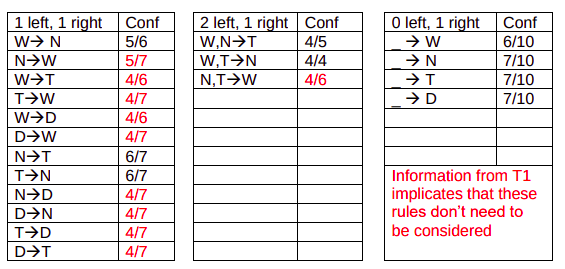
\includegraphics[width=0.6\textwidth]{ruleset.png}
	\end{figure}
	\end{enumerate}
\end{itemize}

\section{Recommendation Systems}
\begin{itemize}
	\item Approaches:
	\begin{itemize}
		\item Association Rules: discover \textbf{correlations}
		\begin{itemize}
			\item product association
			\item user association
			\item combination of both
		\end{itemize}
		\item Collaborative Filtering: discover \textbf{similarity}
		\item Singular Value Decomposition
	\end{itemize}
\end{itemize}

\subsection{Collaborative Filtering}
\begin{itemize}
	\item Idea: 
	\begin{itemize}
		\item maintain a database of \textbf{user's rating} on items.
		\item for a \textbf{given active user}, find other \textbf{similar users} whose \textbf{rating strongly correlates} with the active user.
		
		$\rightarrow$ recommend items highly rated by similar users, which is \textbf{not rated} by active user.
	\end{itemize}
	
\end{itemize}

\subsubsection{Process}
\begin{enumerate}[label= \protect \circled{\arabic*} ]
	\item define \textbf{active user} $a$ and \textbf{other users} $u$.
	\item calculate \textbf{weighted correlation} $w_{a,u}$ based on \textbf{number of co-rated items m} . 
	\begin{itemize}
		\item calculate average of the \textbf{co-rated items} $\bar{r}_a, \bar{r}_u$
		\item calculate the variance $\sigma_{r_{a}}^2, \sigma_{r_{u}}^2$ and standard deviation.
		\item calculate the covariance. \textbf{Don't forget the minus/plus symbol!!!} 
		\item calculate the weighted correlation.
	\end{itemize}
	
	$$w_{a,u} = s_{a,u} \cdot c_{a,u}$$ 
	$$c_{a,u} = \frac{Cov(r_{a}, r_{u})}{\sigma_{r_{a}} \cdot \sigma_{r_{u}}}$$
	$$Cov(r_{a}, r_{u}) = \frac{1}{m-1}\cdot \Sigma (r_a - \bar{r}_a) (r_u - \bar{r}_u)$$
	\item \textbf{rating prediction} for item i for active user.
	\begin{itemize}
		\item calculate \textbf{average rating for all rated items} $\bar{r}_a$ of active user a. 
		\item calculate \textbf{average rating for all rated items} $\bar{r}_u$ of each other user u.
		\item $r_{u,i}$: other user u's rating on the i-th item.
	\end{itemize}
	$$p_{a,i} = \bar{r}_a + \Sigma_{u = 1}^k \dfrac{w_{a,u} \cdot (r_{u,i} - \bar{r}_u)}{\Sigma_{u=1}^k |w_{a,u}|}$$
\end{enumerate}	

\subsubsection{Limitation in Collaborative Filtering}
\begin{itemize}
	\item \textbf{Cold Start}: \textbf{enough users and ratings} are needed to generate recommendations.
	\item \textbf{Sparsity}: the user/rating matrix can be sparse even there are many users 
	
	$\rightarrow$ hard to find \textbf{co-rated} items.
	\item \textbf{First Rater}: with a \textbf{new product}, there must first be consumers who test and evaluate it. 
	\item \textbf{Popularity Bias}: cannot recommend items to users with \textbf{unique taste}. Tend to recommend popular items.
\end{itemize}

$\rightarrow$ Alternative: \textbf{Content-Based Filtering}
\begin{itemize}
	\item idea: based on information of the content of items.
	\item solve: 
	\begin{itemize}
		\item combat popularity bias
		\item combat first rater.
		\item no need of user ratings $\rightarrow$ cold start + sparsity combated.
	\end{itemize}
\end{itemize}

\subsection{Singular Value Decomposition}
\begin{itemize}
	\item Idea: produce a low-dimensional representation of the customer-product space.
	\item Model:
	$$A = U \cdot S \cdot V^T$$
	\begin{itemize}
		\item A: the rating matrix, or the rating we want to predict.
		\item U: maps \textbf{users to concepts}
		\item S: strength of concepts/categories
		\item $V^T$: maps \textbf{venues/products to concepts} 
	\end{itemize}
	\item \textbf{Rating Prediction}: rating for item i from user.
	\begin{itemize}
		\item calculate/consider the average rating of user.
	\end{itemize}
	$$r_{u,i} = \bar{r}_u + U(user) \cdot S \cdot V^T(item)$$
	
	\item Interpretation of values:
	\begin{itemize}
		\item User matrix(U):
		\begin{itemize}
			\item positive: higher interest
			\item negative: lower interest
			\item 0: no interest
		\end{itemize}
		\item Product matrix($V^T$):
		\begin{itemize}
			\item positive: \textbf{positively represented} in the i-th latent factor. Users having preference in i-th latent factor will \textbf{prefer items with positive value over items with negative values}.
			\item negative: \textbf{negatively represented} in the i-th latent factor. Users having preference in i-th latent factor will \textbf{like item less}.
		\end{itemize}
	\end{itemize}
\end{itemize}
